\section{Throughput for Writes (90 pts)\label{sec:4}}

    \begin{table}
        \scriptsize{
            \begin{tabular}{|l|c|}
                \hline Number of servers                & 3 \\
                \hline Number of client machines        & 3 \\
                \hline Instances of memtier per machine & 2 \\
                \hline Threads per memtier instance     & 1 \\
                \hline Virtual clients per thread       & [1, 2, 4, 8, 16, 32, 48] \\
                \hline Workload                         & Write-Only \\
                \hline Multi-Get behavior               & N/A \\
                \hline Multi-Get size                   & N/A \\
                \hline Number of middlewares            & 2 \\
                \hline Worker threads per middleware    & [8, 16, 32, 64]  \\
                \hline
            \end{tabular}
            \caption{Experimental parameters for experiment 4.0.\label{tab:40_setup}}
        }
    \end{table}

    \subsection{Full System\label{subsec:4_full-system}}

        \begin{figure*}
            \vspace*{-.5\baselineskip}
            \makebox[1\linewidth][c]{%
                \centering
                \begin{subfigure}[t!]{0.55\textwidth}
                    \centering
                    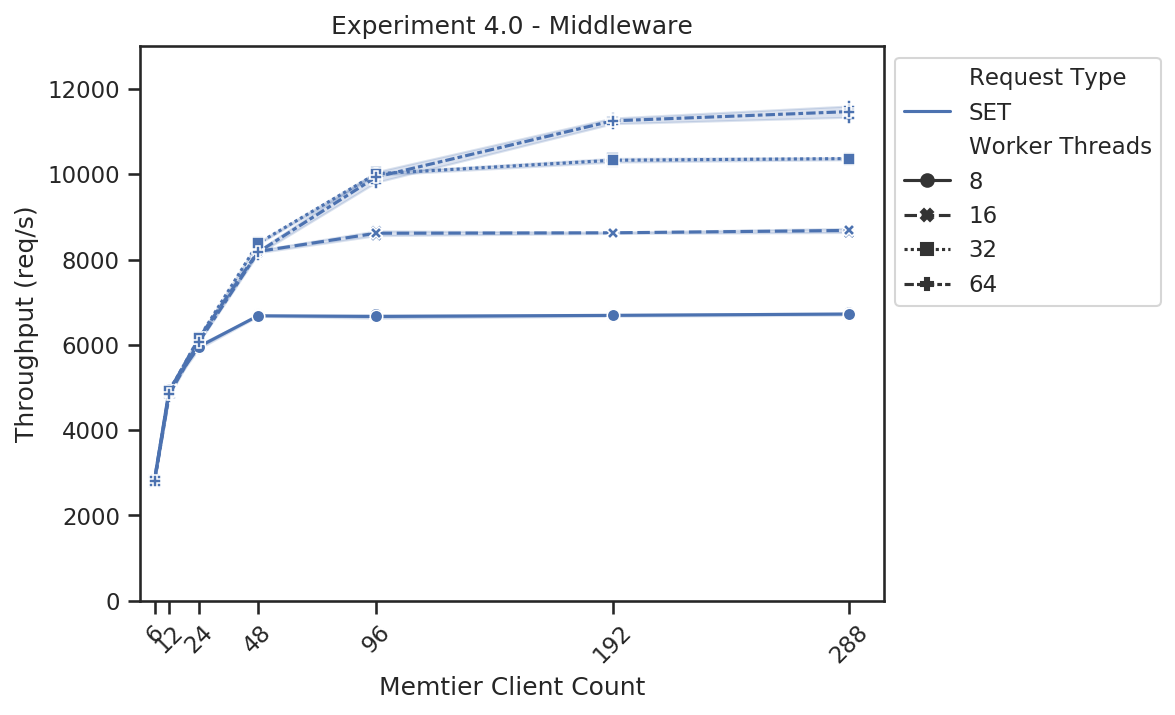
\includegraphics[width=1\textwidth]{../data_analysis/figures/4-0_mw_throughput.png}
                    \caption{Request throughput.\label{fig:sets_mw_tp}}
                \end{subfigure}
                \begin{subfigure}[t!]{0.55\textwidth}
                    \centering
                    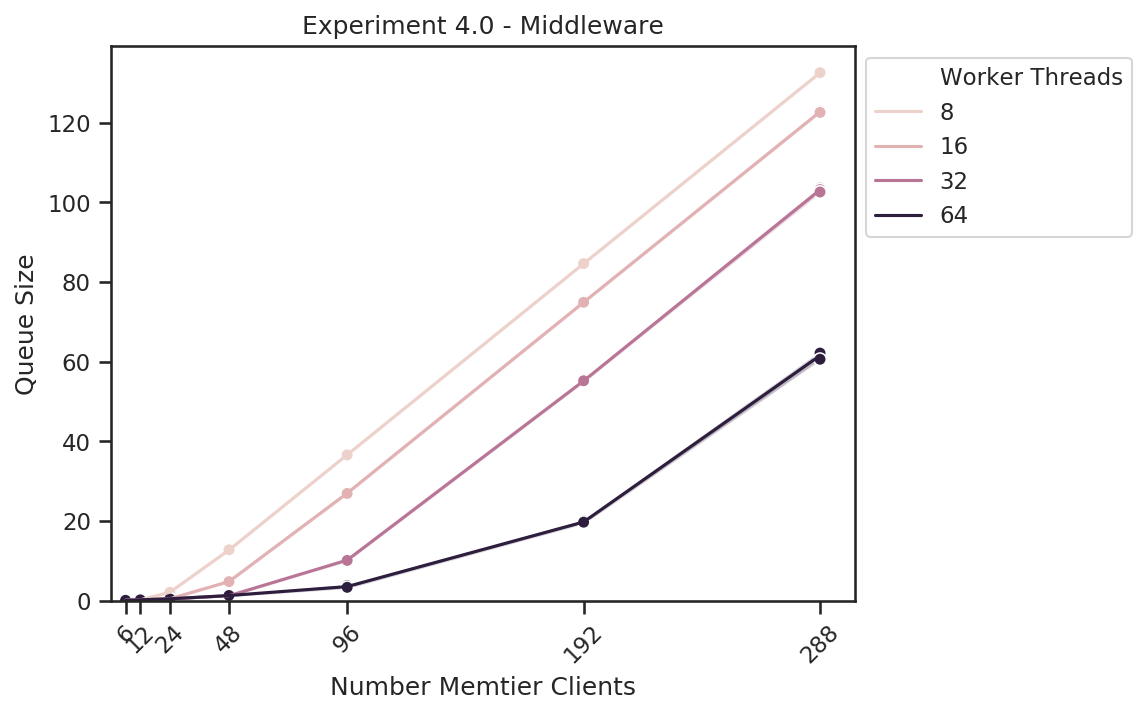
\includegraphics[width=1\textwidth]{../data_analysis/figures/4-0_mw_queue-size.png}
                    \caption{Queue sizes.\label{fig:sets_mw_qs}}
                \end{subfigure}
            }
            \makebox[1\linewidth][c]{%
                \centering
                \begin{subfigure}[t!]{0.55\textwidth}
                    \centering
                    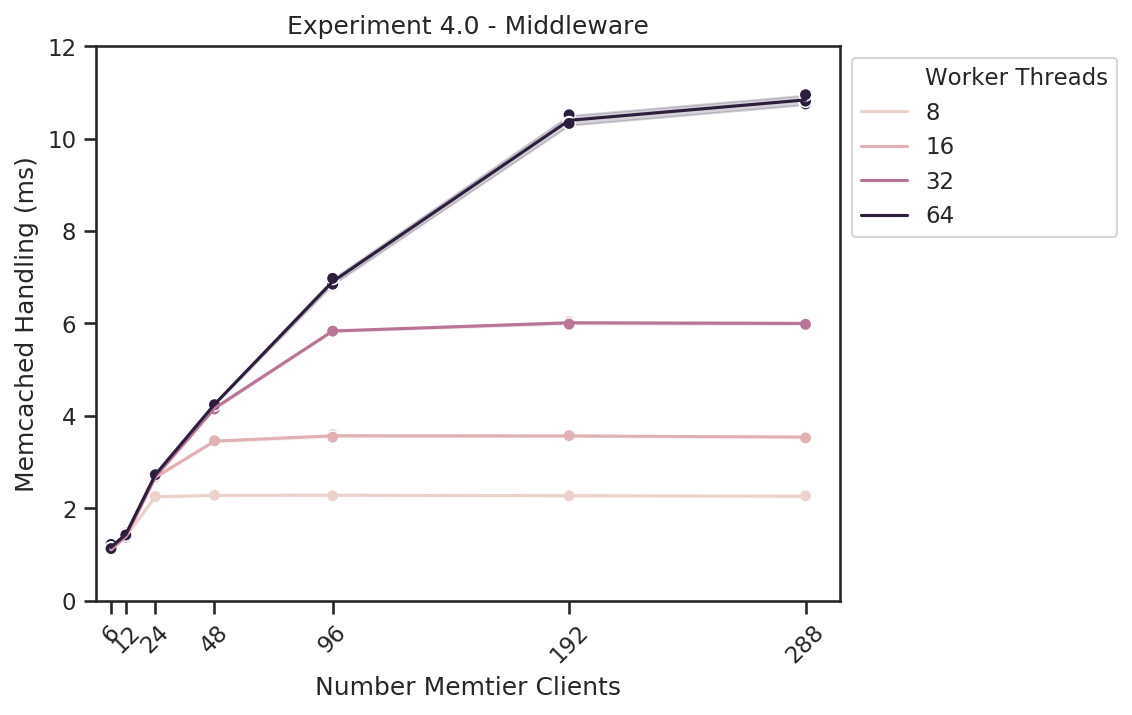
\includegraphics[width=1\textwidth]{../data_analysis/figures/4-0_mw_mc-comm-time.png}
                    \caption{Memcached communication time.\label{fig:sets_mw_mct}}
                \end{subfigure}
                \begin{subfigure}[t!]{0.55\textwidth}
                    \centering
                    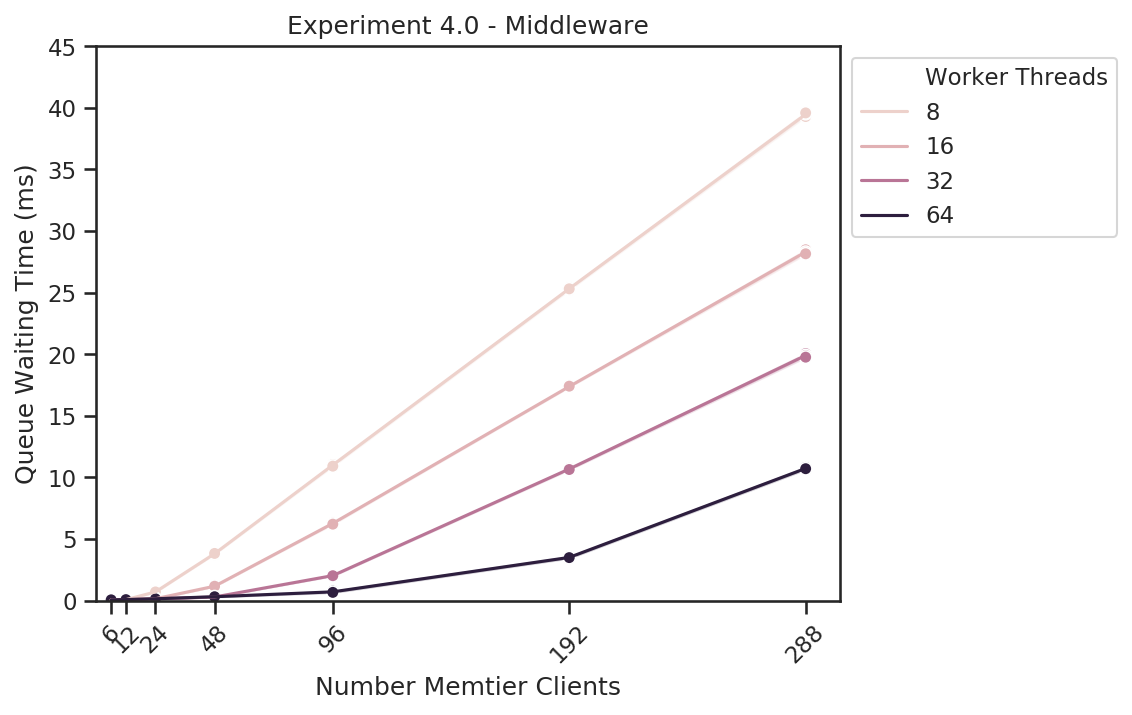
\includegraphics[width=1\textwidth]{../data_analysis/figures/4-0_mw_queue-wait-time.png}
                    \caption{Queue waiting time.\label{fig:sets_mw_qwt}}
                \end{subfigure}
            }
            \makebox[1\linewidth][c]{%
                \centering
                \begin{subfigure}[t!]{0.55\textwidth}
                    \centering
                    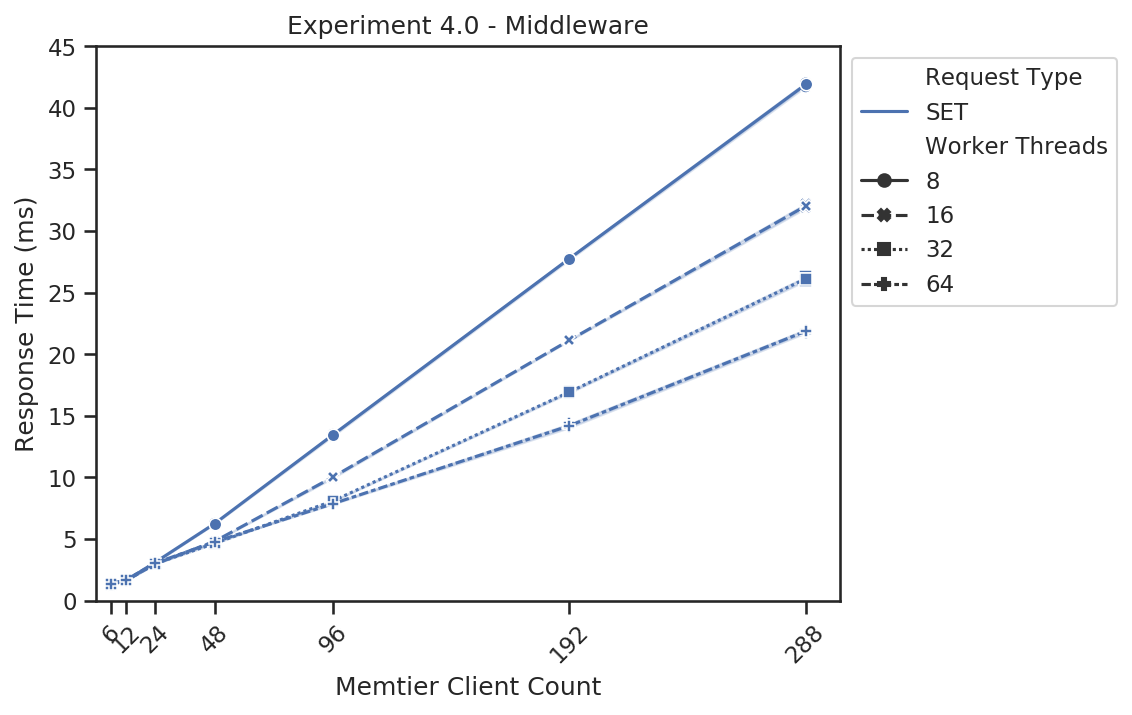
\includegraphics[width=1\textwidth]{../data_analysis/figures/4-0_mw_response_time.png}
                    \caption{Response times.\label{fig:sets_mw_rt}}
                \end{subfigure}
            \caption{\mw{} statistics based on SET requests for various amounts of worker threads and active
                     clients.\label{fig:mw_sets_sll}}
            }
        \end{figure*}

        \subsubsection{Explanation\label{subsubsec:4_full-system_explanation}}

            Compared to experiment \ref{subsec:3_two-middlewares} a decrease in performance can be observed for
            throughput. This follows from the fact that each \mw{} is connecting to three \srv{}s instead of just a
            single one and SETs need to be replicated amongst all connected \srv{}s. It is relevant to recall the design
            of the middleware. It may serve multiple requests at once but each request is handled in a single threaded
            fashion and as such no parallelization for communication between the middleware and memcached occurs.

            As in the previous experiment throughput increases are observed for increasing amounts of worker threads and
            active clients in the system. In the case of 8 worker threads limited gains are observed for 24 clients, no
            gains after 48 clients; 16 worker threads have comparable behaviours for 48 and 96 clients; 32 worker
            threads for 96 and 192 clients and 64 worker threads for 192 and 288 clients. A clear trend can be observed
            thus with saturation points approaching when three times the amount of clients connect to the current
            worker thread configuration and actually reached for four times the amount of worker threads. This reflects
            in the queue sizes seen in figure \ref{fig:sets_mw_qs}. For the aforementioned amount of clients a change in
            steepness can be observed which shows the queue beginning to fill up stronger. As a consequence queue
            waiting times grow which means the overall response time of the system increases. Yet small throughput
            increases are expected as now each worker thread can immediately get an element from the queue without
            having to wait on said queue. This claim assumes the memcached communication time to also stay constant
            between the amounts of clients for limited and no gains. This holds well for configurations of 8\textendash
            32 worker threads. For 64 worker this is not strictly speaking observed but overall the gains of throughput
            are small enough to claim the system is well saturated as indicated by the growing queue.

            One note on the queue size on the previous claim to hold is that the queue must be larger than the amount of
            current worker threads. As such each worker thread has the guarantee to pick up a new task without having
            to wait for said task to be generated.

    \subsection{Summary\label{subsec:4_summary}}

        Based on the experiments above, fill out the following table with the data corresponding to the maximum throughput point for all four worker-thread scenarios.

        \begin{center}
            {Maximum throughput for the full system}
            \begin{tabular}{|l|p{1.5cm}|p{1.5cm}|p{1.5cm}|p{1.5cm}|}
                \hline                                            & WT=8    & WT=16   & WT=32    & WT=64    \\
                \hline Amount of active clients                   & 48      & 96      & 192      & 288      \\
                \hline Throughput (Middleware)                    & 6680.06 & 8615.87 & 10327.67 & 11468.23 \\
                \hline Throughput (Derived from MW response time) & 7674.19 & 9568.57 & 11340.34 & 13171.54 \\
                \hline Throughput (Client)                        & 6675.14 & 8610.97 & 10323.38 & 11462.18 \\
                \hline Average time in queue                      & 3.82    & 6.28    & 10.70    & 10.72    \\
                \hline Average length of queue                    & 10.97   & 23.51   & 50.35    & 56.99    \\
                \hline Average time waiting for memcached         & 2.28    & 3.57    & 6.02     & 10.84    \\
                \hline 
            \end{tabular}
        \end{center}

        The numbers presented are derived applying the reasoning in subsubsection
        \ref{subsubsec:4_full-system_explanation}. It can be observed that the trend to an increase in throughput with
        the amount of worker threads is valid yet at a certain point diminishing returns are to be expected. The
        throughput deltas are (rounded to integers) 1936, 1712 and 1141 and illustrate the point of not scaling linearly
        with the amount of worker threads. Additionally the throughput measured by \mw{}s and \cli{}s match up well. The
        derived throughput from the middleware can be explained as being different by the fact that the interactive law
        applied assumed a thinking time of 0. This obviously is violated for the middleware as each request's response
        time misses out on the communication time and packet handling between memtier and the middleware. A fixed offset
        is not expected to exist as for each given throughput the amount of clients also grows, yet \cli{}s are
        physically only 2 core machines. As such for increasing the number of clients more scheduling overhead is
        expected. This means the interactive law, with no thinking time, applied on the response time derived from the
        middleware is violated. Applying it on the throughput is valid though as a closed system is used. As such the
        throughput and response time are expected to be correlated by taking the inverse to get the respectively other
        metric.

        A note on the queue sizes. They are for all but the case of 64 worker threads above said amount. The system is
        therefore expected to actually be slightly oversaturated for all points whereas for 64 worker threads the point
        of perfect saturation is reached to within a couple percent.

        We can therefore derive that in general between three to four times the amount of clients for worker threads is
        the optimal setup for write only workloads if the minimum amount of threads is to be used. There is no
        measurable loss of performance in adding more worker threads.
